\documentclass[10pt, twocolumn]{article}
\setlength{\columnsep}{0.05\textwidth}
\usepackage[margin=0.7in]{geometry}
\usepackage{graphicx}
\usepackage{float}
\usepackage{hyperref}
\usepackage{amssymb}
\usepackage{amsmath}
\usepackage[]{algorithm2e}
\usepackage{fancyhdr}
\usepackage{dsfont}
\usepackage{textcomp}

\pagestyle{fancy}
\fancyhf{}
\rhead{Mucong Ding}
\lhead{mcding@mit.edu}

\begin{document}

\title{Report of 6.437 Project Part II}

\author{Mucong Ding, mcding@mit.edu, Stu ID: 920494196}


\maketitle

\begin{abstract}
This is the report of project part II of 6.437 in Spring 2018. This report gives a complete description of the decoding methodology and algorithm used in this project. More specifically, all refinements and enhancements designed to improve the basic MCMC algorithm in part I are described. Detailed analyses and evaluations of the improvements are provided, in order to prove their effectiveness. All hyper-parameters are optimized by grid-search. And the performance of the final algorithm is evaluated and compared to the original MCMC algorithm.
\end{abstract}

\section{\label{sec1}Introduction}
\subsection{Problem Description and the Basic Algorithm}
This project aims to design a decoding algorithm for the cipher text encrypted by some secret substitution cipher, a method of encryption by which units of plain text are replaced according to a ciphering function. We only consider substitution cipher which operates on single symbols, and thus the ciphering function $f$ is a permutation on symbols $\mathcal{A}=\{\text{a, b, ..., z, \textvisiblespace, .}\}$. In part I, we use the Metropolis-Hastings algorithm taught in class to develop a simple MCMC-based decoder. However, its decoding accuracy (the number of correctly decoded symbols over the text length, for a specific cipher text) is generally low (on average around $0.7$ in my implementation). And its speed is slow (taking around 10s for a single trial with 10000 iterations), even all math computations are implemented under \textit{numpy} back-end.

\subsection{Proposed Enhancements}
In part II, we aimed to improve the accuracy and speed of the basic MCMC-based algorithm. I proposed several important changes, listed as follows:
\begin{itemize}
	\item \textbf{Fast Ensemble MCMC}: run multiple MCMC samplers in parallel, speedup by \textit{numpy} matrix operations and some tricks and simplifications of the original MH algorithm, dramatically increase the low performance caused by bad initialization
	\item \textbf{Refined Language Model}: use symbol, bigram, trigram and word probabilities to model the likelihood of an English text, solve the small acceptance rate problem and speedup convergence
	\item \textbf{Linear Assignment Initialization}: use the solution of a linear assignment problem to initialize the guesses, achieve around $0.4$ accuracy before running MCMC-based algorithm, solve the assignment problem quickly by the Hungarian method, speedup the convergence
	\item \textbf{Majority Voting and Mapping Fixing}: use the majority mapping (ciphering function) instead of the most probable one as the final output, fix a part of the mapping along the progression of the MCMC-algorithm by majority voting to speedup the convergence
\end{itemize}
Detailed descriptions of the 4 improvements can be found in later sections.

\subsection{Analyses and Evaluations}
I analyze the effectiveness and contributions of each improvements individually, by comparing the accuracy and runtime of algorithms with/without this enhancements. The evaluation results are described in later sections, which prove the usefulness of each enhancement methodology.

Moreover, for different combinations of the methodologies, I evaluate the performance of each algorithm by some more completed metrics, including the Kendall tau distance and error map. The Kendal tau distance is a direct indicator of the number of swaps to the ground-truth mapping. The error map is very useful to reveal the weaknesses of language models.

\subsection{Hyper-parameter Tuning and The Final Decoder}
There are a couple of hyper-parameters (mainly from the language model and the mapping-fixing mechanism), which could be fine-tuned to optimize the performance of the final algorithm. I use grid-search to find a good combination of these hyper-parameters. This process is described in later sections.

The final decoder is a MCMC-based algorithm will all of the 4 refinements and a set of fine-tuned hyper-parameters. We analyze its performance in detail and compare to the original one.

\subsection{Structure of The Report}
This report is structured as follows:
\begin{itemize}
	\item \textbf{Section \ref{sec1}: Introduction}: problem and background, listing of improvements, listing of the analyses and evaluations
	\item \textbf{Section \ref{sec2}: Enhancement}: detailed description of each enhancement methodology along with evaluations to prove their effectivenesses
	\item \textbf{Section \ref{sec3}: Analysis and Conclusion}: hyper-parameter tuning, analyses of the final algorithm
\end{itemize}


\section{\label{sec2} Enhancement}
\subsection{\label{subsec2.1}Fast Ensemble MCMC}
We can consider the solution space of $28!$ candidates as a big graph, where each node is a mapping, and two nodes are connected if one can be transformed to another with a single swapping. The MCMC sampler is a random-walker on this graph. Since he diameter of this graph is $28$, it is likely that some local maximum (in terms of the likelihood function) exist. One single sample is likely to be kept by local maximum and be affected by bad initialization. The direct solution to this is to run multiple samplers in parallel. If we denote the number of samplers by $m$, we usually take $m\sim10^1$

Most of the computations with multiple samplers can be designed as matrix operations and arithmetics. For the computation of n-gram log probabilities (some of the log probabilities of n-gramas in the deciphered text, for a specific n), we speedup the process by pre-computing the n-gram frequency matrices of the cipher text. Since the deciphering function is merely a permutation of symbols, the n-gram frequency matrix of the deciphered text is a permutation of the per-computed one, and is simply a view of the per-computed matrix with advanced indexing. Then, calculation of the sum log probability is carried out as a dot-product of the frequency matrix and the log-probabilities matrix. If we denote the length of cipher text as $l$ and the number of symbols as $n=28$, the running time of a single iteration of one sampler is $\mathcal{O}(n^3)$ (since I use up to trigrams) instead of $\mathcal{O}(l)$. For usual text, $l>1000$, the former one is faster, which takes 382\textmu s for one sampler in one iteration. The latter one uses 571\textmu s.

The MH algorithm is also simplified to save time. Since generating random number expensive, and the ratio between two likelihoods is usually far from $1$ (i.e. not similar in terms of the magnitudes). The acceptance probability defined as $\alpha(x^n, x^{n-1})=\min\{1, \mathcal{L}(x^n)/\mathcal{L}(x^{n-1})\}$ is usually either 1 or very close to 0. Thus, it does not hurt to change the definition to $\alpha(x^n, x^{n-1})=\mathds{1}_{\mathcal{L}(x^n)>\mathcal{L}(x^{n-1})}$. The latter definition will be evaluated much faster. In my implementation, one state transition of one sampler (not counting the part of likelihood calculation) using the former definition takes 2.87\textmu s, while the latter one takes only 74.7ns. We call the simplified one as the fast version.

The running time of the vectorized implementation of the fast ensemble MCMC algorithm scales linearly in $m$, the number of samplers, as shown in Fig. \ref{fig:ensemble_cal_time}. Thus it's faster than running multiple trials one by one for any $m$.
\begin{figure}[t]
	\centering
	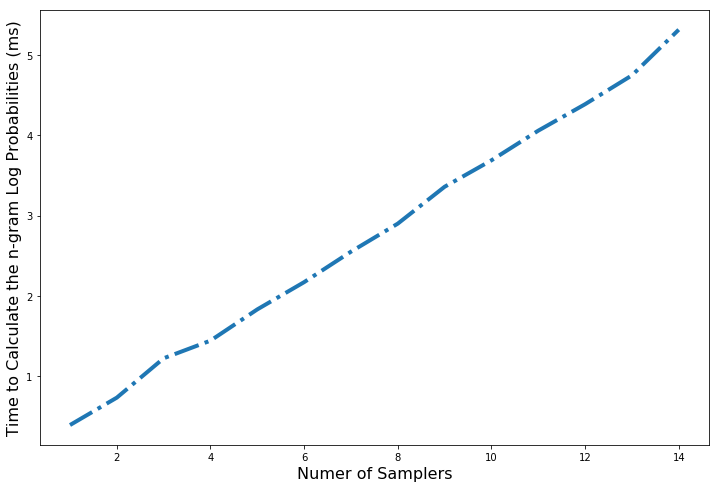
\includegraphics[width=0.9\linewidth]{pics/ensemble_cal_time.png}
	\caption{Running time of vectorized n-gram log probability calculation function versus the number of samplers}
	\label{fig:ensemble_cal_time}
\end{figure}

\subsection{\label{subsec2.2}Refined Language Model}
In part I, we modeled the English texts as Markov Chains, whose likelihood function is: $\mathcal{L}(x) = \mathcal{P}_{x_1}\Pi_{i=1}^{n-1}\mathcal{P}_{x_i, x_{i+1}}$, where $\mathcal{P}_{a}$ is the probability of symbol $a$ and $\mathcal{P}_{a, b}$ is the probability of bigram $ab$. Using this likelihood definition, we plot the error map of the ensemble of mappings, as shown in Fig. \ref{fig:error_map_mc}.
\begin{figure}[t]
	\centering
	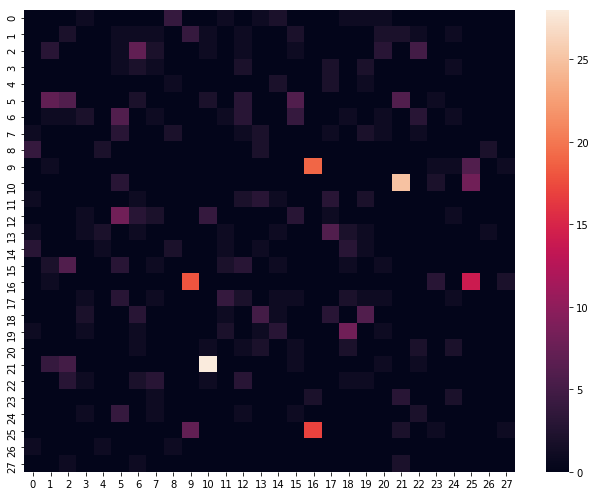
\includegraphics[width=0.9\linewidth]{pics/error_map_mc.png}
	\caption{Error map of 50 sampler with Markov Chain likelihood when decoding accuracy is around $0.75$, the y-axis is the index of ground-truth symbol, the x-axis is the index of deciphered symbol, the color represents the number of mis-decryption in this ensemble.}
	\label{fig:error_map_mc}
\end{figure}
Where we can infer from the 4 orange-dots, that $j$ is often mis-decrypted as $i$ and $z$, and vise-versa. However, we know $\mathcal{P}_{j}=0.0016<<\mathcal{P}_{i}=0.0757$, i.e., they could be distinguished merely using the symbol probabilities.

This inspires me that a simple and direct refinement of the Markov Chain model is to define the likelihood function as $\mathcal{L}(x) = \mathcal{L}_1(x)\mathcal{L}_2(x) = \Pi_{i=1}^{n}\mathcal{P}_{x_i}\Pi_{i=1}^{n-1}\mathcal{P}_{x_i, x_{i+1}}$, where $\mathcal{L}_1$ is the likelihood modeled using only symbol probabilities, and $\mathcal{L}_2$ only uses bigram probabilities. The error map of ensembles with the same size revolved under this definition is like Fig. \ref{fig:error_map_refined}.
\begin{figure}[t]
	\centering
	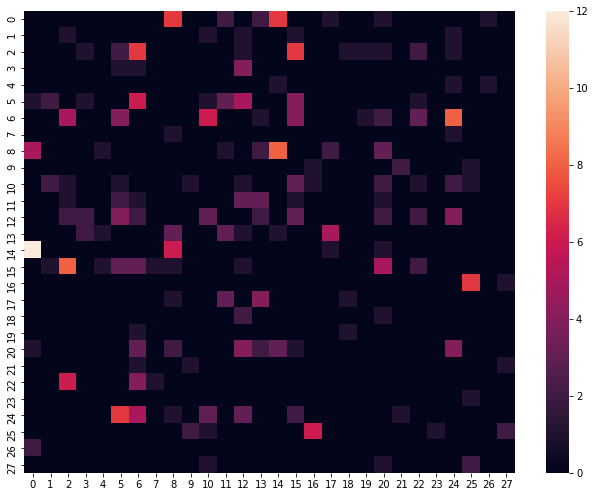
\includegraphics[width=0.9\linewidth]{pics/error_map_refined.png}
	\caption{Error map of 50 sampler with refined likelihood when decoding accuracy is around $0.75$, the y-axis is the index of ground-truth symbol, the x-axis is the index of deciphered symbol, the color represents the number of mis-decryption in this ensemble.}
	\label{fig:error_map_refined}
\end{figure}
Where we can see now the most common mis-decryption is from $n$ to $a$, this is acceptable since $\mathcal{P}_{a}=0.0804\approx\mathcal{P}_{n}=0.0723$.

To further enrich our language model, we use up to trigram probabilities $\mathcal{P}_{a,b,c}$ for trigram $abc$, that is to say, $\mathcal{L}(x) = \mathcal{L}_1(x)\mathcal{L}_2(x)\mathcal{L}_3(x) = \Pi_{i=1}^{n}\mathcal{P}_{x_i}\Pi_{i=1}^{n-1}\mathcal{P}_{x_i, x_{i+1}}\Pi_{i=1}^{n-2}\mathcal{P}_{x_i, x_{i+1}, x_{i+2}}$, where $\mathcal{L}_3$ is the corresponding trigram likelihood. The MCMC-based algorithm with this likelihood function can already achieve 0.92 decoding accuracy on average. Note that the trigram probabilities data from \url{http://norvig.com/mayzner.html} does not contains the space and dot symbols. I estimate the probabilities of trigrams containing spaces and dots by the 13k character plain text provided in the project.

Moreover, in order to further increase the decoding accuracy, we can use a word dictionary to check the deciphered text. With the linear assignment initialization (see \ref{subsec2.3}), we can decode space and dot correctly at the very early stage of MCMC-algorithm, then it make sense to split the deciphered words and check their validity by the dictionary. The corresponding likelihood is defined as $\mathcal{L}_{w}(x) = \Pi_{w\text{ in }x}\mathcal{P}^{\text{word}}_w$. In practice, $\mathcal{P}^{\text{word}}$ is not a probability function as I set $\mathcal{P}^{\text{word}}_w = \mathcal{P}^{\text{word}}_0 \sim 10^{-40}$ if $w$ is not an English word. And I penalize the case when space and dot is not decrypted correctly as if there are less than $kl$ words in a text $x$ of length $l$, set $\mathcal{L}_{w}(x) = (\mathcal{P}^{\text{word}}_0)^{kl}$. Usually, k is set to $k\approx\frac{1}{10}$.

So that we conclude that our complete enhanced language model use likelihood function $\mathcal{L}(x) = \mathcal{L}_2(x)\mathcal{L}_3^{\mathrm{w}_1}(x)\mathcal{L}_{w}^{\mathrm{w}_2}(x)$. Note $\mathcal{L}_1(x)$ is finally removed since with linear assignment initialization (see \ref{subsec2.3}), it is no longer useful. Note $\mathrm{w}_1$ and $\mathrm{w}_2$ are two constant weight factors, which will be tuned in \ref{sec3}.


\subsection{\label{subsec2.3}Linear Assignment Initialization}
Instead of randomly initialize the candidate mappings, it is much better to initialize them according to the solution of a linear assignment problem.

Consider a cost matrix $C$ where $C_{i, j}$ is the cost of assigning (ciphering) $i$ to $j$. And the total cost is $\Sigma_{i}C_{i, f(i)}$, where $f$ is a permutation (ciphering function). The linear assignment problem solves the mapping $f$ which minimizes the optimal cost. If we define our cost as: $C_{i, j} = (\mathcal{P}_{i} - \mathcal{F}_{f(i)})^2$, where $\mathcal{P}_{i}$ is the symbol probability of symbol $i$ and $\mathcal{F}_{j}$ is th normalized symbol frequency of symbol $j$ in the cipher text. Then, this linear cost is the sum of squared errors of the estimated symbol probabilities of the deciphered text. Solving this assignment problem give us the permutation $f$ which satisfies the symbol probability distribution most.

The Hungarian algorithm can be used to solve this linear assignment problem in polynomial time, that is $\mathcal{O}(p(n))$ where $n=28$ is the size of alphabets. Although it's a little bit expensive, we only need to run it once. On top of the optimal $f$, we can add some randomness by randomly swap two symbols in the permutation, for each sampler. In general, the decoding accuracy merely after initialization is dramatically increased, from $0.04\pm0.016$  to $0.32\pm0.082$, for random cipher text of length $l=1000$. And as a consequence, the convergence time of MCMC-algorithm reduces by around 10s when $m=10$ (10 samplers) with the linear assignment initialization.

\subsection{\label{subsec2.4}Majority Voting and Mapping Fixing}
For the ensemble MCMC-algorithm, what should be the final output? A natrual idea is the mapping with largest likelihood in the ensemble. However, it is found that even with refined modeling, for some text, the correct ciphering function does not have the largest corresponding likelihood. We can apply majority voting here. Define a hyper-parameter $t\in(0.5,1]$ and for a set of candidate ciphering functions $f_1, \cdots, f_m$ and for a ciphered symbol $i$, we decoded it to $j$ if more than $tm$ ciphering functions satisfies $f_i^{-1}(i) = j$ for $i\in\{1, \cdots, m\}$. Correspondingly, we can define a majority mapping $f$ where $f(j) = i$. Please note that $f$ must be a permutation, since more than a half $f_i$ satisfies the same mapping for each symbol, we can see for $i_1\neq i_2$, $f^{-1}(i_1) = j_1 \neq j_2 = f^{-1}(i_2)$, otherwise there must exist some $f_i$ which satisfies $f^{-1}(i_1) = f^{-1}(i_2)$ contradicts to the fact that $f_i$ is a permutation. Thus the majority voted mapping is really a permutation. Using the majority voted mapping instead of the most probable mapping slightly increases the decoding accuracy, up to $0.02$ when $m=10$ and $t=0.8$. Furthermore, it gives us a natural termination condition: terminating the algorithm when the majority mapping $f$ can be defined, that it, for every symbol $i$, there is a valid majority vote among $f_i^{-1}$. In practice, we also define a upper limit of iterations to run, which is usually set to $3000\sim5000$.

Another idea of using majority voting to speed up the convergence is called mapping fixing. That is, if for a specific $i$, if the majority vote appears and is stable for some number of iterations (usually set to $100\sim200$), we consider it as already convergent and no longer allow state transitions (swapping) that will change this mapping. That is, the effective number of neighbors of a state is reducing, along with the progression of the algorithm. This helps the algorithm converge faster and achieve a high acceptance rate in the later stage of a session. With $m=10$ samplers and $t=0.8$, this mapping fixing mechanism can speedup the running time from $34\pm9s$ to $14\pm4s$. And for $t>=0.8$, the accuracy will not be notably affected. An overhead of this mechanism is that we have more complexed functions for proposing swapping (state-transitions), however, the delta running-time in this part is much more smaller than the computation of likelihood functions. Thus the running-time per iterations will not be notably larger as well.

\section{\label{sec3} Analysis and Conclusion}
\subsection{\label{subsec3.1}Hyper-Parameter Tuning}
To summarize, we list all the hyper-parameters appear above, they are: $m$ (number of samplers), $\mathrm{w}_1$, $\mathrm{w}_2$ (two likelihood weights) and $t$ (majority voting threshold). Actually, there are a lot more hyper-parameters hidden in the algorithm, but as they are not as important as these 4, we ignore the tuning process of them.

Tuning these 4 hyper-parameter is not very hard. For $m$, to reach a reasonable running time and acceptable accuracy, we can only choose $10\leq m\leq30$, and correspondingly $0.8\leq t \leq 0.9$. Since my algorithm isn't very fast, I prefer to achieve higher accuracy even risking to increase the running time. So I choose $m=20$ with $t=0.9$.

For $\mathrm{w}_1$, $\mathrm{w}_2$, I simply use grid-searching to find the best combination, and the result is $\mathrm{w}_1=0.3$ and $\mathrm{w}_2=16$. Not surprisingly, it is the number where $\mathcal{L}_2(x) \sim \mathcal{L}_3^{\mathrm{w}_1}(x) \sim \mathcal{L}_{w}^{\mathrm{w}_2}(x)$.

\subsection{\label{subsec3.2} Final Evaluation and Conclusion}
The final algorithm is the combination of basic MH algorithm and the 4 improvements. Generally, it can terminate in $22\pm8$s with $98\pm3\%$ accuracy.

I believe there are a lot more extensions and refinements can be done on this MCMC-based algorithm. Which could be further investigated in the future.

\end{document}
